\documentclass[main.tex]{subfiles}

%\newpage
\begin{document}

%\begin{SCfigure}
%    \centering
%    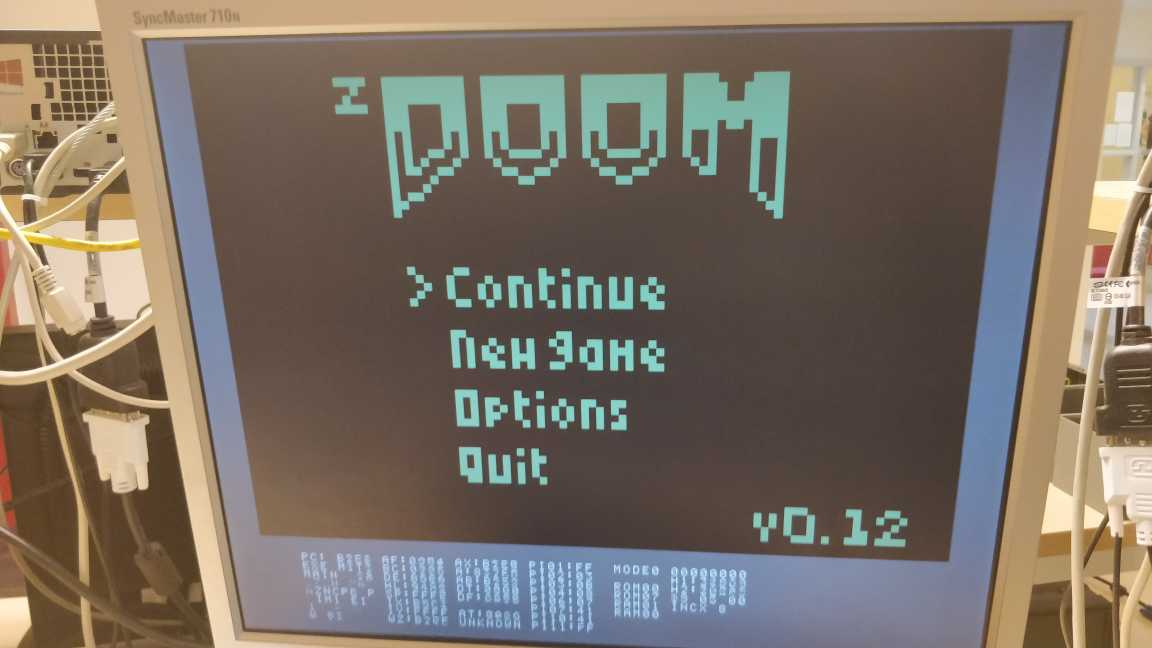
\includegraphics[width=0.8\textwidth,bb=0 0 1152 648]{img/monitor_small.jpg}
%    \caption{Konstruktionens display vid körning av spelet zDoom.}
%\end{SCfigure}

\section{Konstruktion}
Konstruktionen har använt ett Nexys3-kort med en Spartan6 FPGA från Digilent
som designen programmeras till. Utöver FPGA:n används även RAM-minnet på kortet
samt knappar, strömbrytare och dess 7-segments-display.

Kortet är kopplat till en dator som tillför ström och programmerar bitfilen
till FPGA:n på kortet. Datorn används även för att skriva program till RAM.
Ett PS/2 tangentbord är kopplat till FPGA-kortets USB-port och en VGA-skärm
till dess VGA-port.  

\begin{SCfigure}
    \centering
    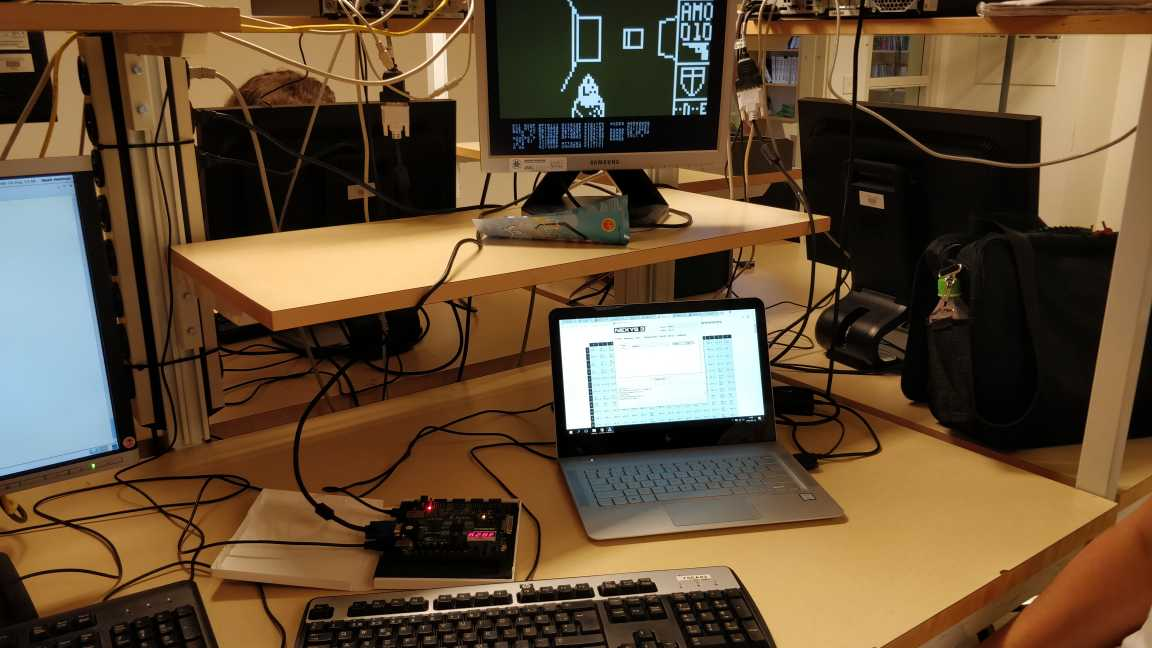
\includegraphics[width=0.8\textwidth,bb=0 0 1152 648]{img/setup_small.jpg}
    \caption{VGA-skärm och tangentbord kopplat till FPGA-kort tillsammans med
    laptop som används för att programmera FPGA:n samt ladda program till
    minnet.}
\end{SCfigure}

\subsection{Ladda program}
För att ladda program till kortets RAM har programmet ``Digilent Adept''
använts. För att ladda en fil till minnet väljs RAM under fliken {\it Memory}.
Därefter väljs filen under {\it Write File To Memory} och skrivs till minnet
när {\it Write} trycks. Därefter kan bitfilen laddas under fliken {\it Config}.
Bitfilen väljs och programmeras därefter genom att trycka på {\it Program}. Då
kommer processorn sätta igång och börja exekvera på adress \mono{0x8000}.

Vid laddning till minnet kan en startadress väljas. Om ett program som startar
i början av filen ska laddas bör det läggas på adressen \mono{0x7c000} eftersom
\mono{0x8000} leder dit med den minnesmappning som är inställd vid uppstart. Om
en hel ROM-dump ska laddas såsom TI-83p:s operativsystem ska den läggas på
adress \mono{0x00000} eftersom miniräknarens ROM börjar på där. Hur
miniräknarens minne ligger i det fysiska minnet beskrivs i sektion
\ref{sec:mmap} på sidan \pageref{sec:mmap}.

Om ett ROM laddas kommer den hamna i halt-läge och vänta på att användaren
trycker på ON-knappen. ON-knappen är vänster Ctrl på PS/2-tangentbordet.

\subsection{Gränssnitt}
Alla miniräknarens tangenter är kartlagda 1:1 till olika tangenter på
tangentbordet. Se tabell \ref{app:kbd} för vilka knappar som är bundna till
vilka.

CPU:n kan även kontrolleras direkt med hjälp av instrumenten som befinner sig
på kortet. Figur \ref{fig:interface} visar vad de olika instrumenten på kortet
används till. De olika brytarna justerar bland annat lägen och frekvenser. När
alla brytare är nere kör processorn som vanligt på \SI{6}{\mega\hertz}.

\begin{figure}[b]
    \centering
    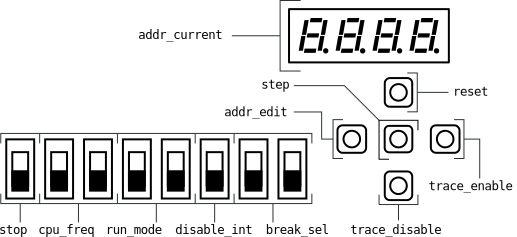
\includegraphics[width=0.7\textwidth]{board.eps}
    \caption{Användning av de olika instrumenten på Nexys3.}
    \label{fig:interface}
\end{figure}

\begin{labeling}{indentzzzzzzzzz}
\item[\mono{stop}]
    Aktivera för att stanna CPU:n och TI-ASIC:en.
\item[\mono{cpu\_freq}]
    Välj processorns frekvens enligt
    \begin{tabular}{rrrr}
        \mono{00}: & \SI{6}{\mega\hertz}, &
        \mono{01}: & \SI{14}{\mega\hertz}, \\
        \mono{10}: & \SI{1}{\mega\hertz}, &
        \mono{11}: & \SI{10}{\kilo\hertz}.
    \end{tabular}
\item[\mono{run\_mode}]
    Välj läge enligt
    \begin{tabular}{rl}
        \mono{00}: & kör processorn normalt, \\
        \mono{01}: & kör en maskincykel i taget, \\
        \mono{10}: & kör en instruktion i taget, \\
        \mono{11}: & kör en T-cykel i taget.
    \end{tabular}
\item[\mono{step}]
    Fortsätter processorn efter brytning. Används för att stega igenom
    instruktioner eller för att fortsätta efter en brytpunkt.
\item[\mono{disable\_int}]
    Förhindra avbrott, \mono{int}-signalen går aldrig aktiv om denna är på.
\item[\mono{break\_sel}]
    Välj brytpunkt enligt
    \begin{tabular}{rl}
        \mono{00}: & ingen, \\
        \mono{01}: & exekvering från vald adress, \\
        \mono{10}: & läsning från vald adress, \\
        \mono{11}: & skrivning till vald adress.
    \end{tabular}
\item[\mono{addr\_edit}]
    En adress kan väljas genom att trycka på \mono{addr\_edit}. Därefter väljs
    siffra med vänster och högerknapp. Adressen visas på 7-segments-displayen.
    En punkt visas intill den siffra som är vald. Siffran kan ökas eller
    minskas med upp och nedknapparna. När adressen är inställd trycks
    mittknappen ner och punkten försvinner.
\item[\mono{reset}]
    Återställer processorn och ASIC:ens alla register och vippor som vid
    uppstart. Processorn börjar då exekvera från adress \mono{0x8000} igen.
    Bildminnet i LCD-kontrollern påverkas dock inte.
\item[\mono{trace\_enable}]
    Aktiverar spårning av alla hopp som processorn utför. Varje gång ett hopp
    utförs stoppas processorn tillfälligt och dess nuvarande adress och dess
    destinationsadress skrivs till det fysiska minnet på adress \mono{0x88000}.
    Efter att ett program har kommit fel kan processorn stoppas och minnet
    läsas med hjälp av programmet Adept. Därefter kan datan enkelt tolkas med
    hjälp av \mono{hexdump} med kommandot
    \lstinputlisting{lst/trc_command.sh}
    som exempelvis ger utdatan
    \lstinputlisting{lst/trc_output.sh}
    Exemplet är från när operativsystemet precis har startat och hamnat i
    halt-läge på adress \mono{0x0aad}. När användaren då trycker på ON-knappen
    sker ett avbrott och processorn hoppar till adress \mono{0x0038} och
    påbörjar avbrottsrutinen.
\item[\mono{trace\_disable}]
    Stänger av spårning så att processorn inte stoppas vid hopp. Återställer
    även pekaren som bestämmer var nästa adress ska skrivas till
    \mono{0x88000}.
\end{labeling}

\clearpage
\end{document}
